% 3.1 =============== 随机最优增长 Edmond ===============

\section{引例：随机最优增长}    \label{sec-eg-opg-growth}

本节对随机最优增长模型（Stochastic Optimal Growth Model / Stochastic Neoclassical Growth Model）进行介绍。
一方面，自Brock and Mirman（1972）首次将随机TFP冲击引入计划者问题，将其作为宏观变量内生波动的解释后，
随机最优增长模型就逐渐成为几乎所有经济周期模型的基本框架。
另一方面，以随机最优增长作为引例，我们将说明外生冲击给模型计算带来的难点，并初步窥探相应数值方法的运用。


% 3.1.1 ===== 基本概念与模型设定 =====
\subsection{基本概念与模型设定}

在确定性模型中，给定期初资本存量，生产函数是确定的，代表性家庭（计划者）面临的资源约束为：
\begin{equation*}
    c_t + k_{t+1} \leq f(k_t)+\left(1-\delta\right)k_t
\end{equation*}

随机最优增长模型与确定性模型的核心区别在于生产函数面临\textbf{随机事件}（Stochastic Event）给生产率带来的不确定性，
资源约束形式为：
\begin{equation*}  
    c_t\left(s^t\right)+k_{t+1}\left(s^t\right) \leq z_t\left(s^t\right) f\left(k_t\left(s^{t-1}\right)\right)
    +\left(1-\delta\right)k_t\left(s^{t-1}\right), \quad \forall s^t
\end{equation*}
其中，称$s_t\in S$是$t$时刻实现的一个随机事件，$S$是随机过程的状态空间（或称为支撑），
称$s^t\equiv \left(s_0,s_1,\cdots,s_t\right)=\left(s^{t-1},s_t\right)$为至$t$时刻已经实现的事件的\textbf{历史}。
举例来看，假设$s_t\in\{0,1\}$，例如$s_t=1$对应高生产率的$z$，$s_t=0$对应低生产率的$z$。
\cref{event-tree}给出了这一情形下（即$S=\{0,1\}$）随机事件可能的展开路径。
从$t=0$时刻看，时刻$t$时历史$s^t$实现的\textbf{无条件概率}为$\pi_t\left(s^t\right)$；
对$t>\tau$，$z^t$实现的\textbf{条件概率}为$\pi_t\left(s^t\mid s^{\tau}\right)$。
\begin{figure}
    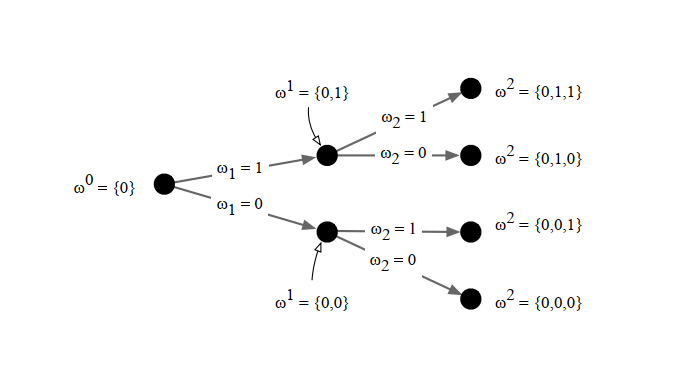
\includegraphics[width=1\textwidth]{figures/part1/ch3/event-tree.png}
    \caption{随机事件树}
    \label{event-tree}
\end{figure}

不失一般性，假设$s_t$在离散空间上取值。从而模型中代表性家庭（计划者）偏好可写为：
\footnote{为了形式的方便，我们通常使用$\mathbb{E}_0$表示基于零时刻给定状态$z_0$下的期望效用}
\begin{equation}    \label{eq-s-opt-growth-preference}
    \begin{aligned}
        U &= \sum_{t=0}^{\infty} \sum_{s^t} \beta^t u\left(c_t\left(s^t\right)\right) \pi_t\left(s^t\right) \\
        &= \mathbb{E}_0 \sum_{t=0}^{\infty} \beta^t u\left(c_t\right)
    \end{aligned}
\end{equation}


% 3.1.2 ===== Edmond =====
\subsection{序列问题和状态依存计划}

在确定性问题中，家庭的最优选择一个\textbf{确定性的序列}；
而在随机问题中，家庭的最优选择依赖于随机过程$z_t$，因此选择的消费和资本序列
$\{c_t\left(z^t\right)\}_{t=0}^{\infty},~ \{k_{t+1}\left(z^t\right)\}_{t=0}^{\infty}$也是随机过程，
通常我们将其称为\textbf{状态依存计划}（Contingent Plans）。我们将先利用序列方法求解状态依存计划的最优条件。

在序列问题下，家庭将概率序列$\pi_t\left(s^t\right)$视为给定，选择消费和资本序列来最大化自身期望效用\ref{eq-s-opt-growth-preference}：
\begin{equation*}
    \max _{\left\{c_t\left(s^t\right), k_{t+1}\left(s^t\right)\right\}_{t=0}^{\infty}} 
        \sum_{t=0}^{\infty} \sum_{s^t} \beta^t u\left(c_t\left(s^t\right)\right) \pi_t\left(s^t\right)
\end{equation*}
资源约束为：
\begin{equation}    \label{eq-s-opt-growth-rc}
    c_t\left(s^t\right)+k_{t+1}\left(s^t\right) \leq z_t\left(s^t\right) f\left(k_t\left(s^{t-1}\right)\right)
        + \left(1-\delta\right)k_t\left(s^{t-1}\right), \quad \forall s^t
\end{equation}
非负性约束为：
\begin{equation*}
    c_t\left(s^t\right), k_{t+1}\left(s^t\right) \geq 0, \quad \forall s^t
\end{equation*}
其中第0期的资本$k_0$和状态$s_0$给定，即$\pi_0\left(s_0\right)=1$。
记与资源约束相关的拉格朗日乘子为$\lambda_t\left(s^t\right)$，则拉格朗日函数为：
\begin{equation*}
    \begin{aligned}
        \mathcal{L} &=\sum_{t=0}^{\infty} \sum_{s^t} \beta^t u\left(c_t\left(s^t\right)\right) \pi_t\left(s^t\right) \\
            &+\sum_{t=0}^{\infty} \sum_{s^t} \lambda_t\left(s^t\right)
            \left[z_t\left(s^t\right)f\left(k_t\left(s^{t-1}\right)\right)+\left(1-\delta\right)k_t\left(s^{t-1}\right)
            -c_t\left(s^t\right)-k_{t+1}\left(s^t\right)\right]
    \end{aligned}
\end{equation*}
容易得到,关于$c_t\left(s^t\right)$的一阶条件为：
\begin{equation}    \label{eq-s-opt-growth-foc-c-sq}
    \beta^t \pi_t\left(s^t\right) u^{\prime}\left(c_t\left(s^t\right)\right)=\lambda_t\left(s^t\right)
\end{equation}
关于$k_{t+1}\left(s^t\right)$的一阶条件为：
\begin{equation}    \label{eq-s-opt-growth-foc-k-sq}
    \lambda_t\left(s^t\right)=\sum_{s^{t+1} \mid s^t} \lambda_{t+1}\left(s^{t+1}\right)
        \left[z_{t+1}\left(s^{t+1}\right)f^{\prime}\left(k_{t+1}\left(s^t\right)\right)+\left(1-\delta\right)\right]
\end{equation}
这里的一个关键点在于：当前$k_{t+1}\left(s^t\right)$的选择会影响$t+1$时刻基于$s^t$的所有可能的$s^{t+1}$下的生产，
反映为求和符号下的$s^{t+1} \mid s^t$。
结合两个一阶条件，可以写出\textbf{随机形式的消费欧拉方程}：
\begin{equation}    \label{eq-s-opt-growth-euler1-sq}
    u^{\prime}\left(c_t\left(s^t\right)\right) = 
        \beta\sum_{s^{t+1}\mid s^t} \pi_{t+1}\left(s^{t+1}\mid s^t\right) u^{\prime}\left(c_{t+1}\left(s^{t+1}\right)\right)
            \left[z_{t+1}\left(s^{t+1}\right) f^{\prime}\left(k_{t+1}\left(s^t\right)\right)+\left(1-\delta\right)\right] 
\end{equation}
其中条件概率$\pi_{t+1}\left(s^{t+1}\mid s^t\right) =\pi_{t+1}\left(s^{t+1}\right)/\pi_t\left(s^t\right)$。
因此，方程右侧是一个\textbf{条件期望}，我们习惯将其写为：
\begin{equation}    \label{eq-s-opt-growth-euler2-sq}
    u^{\prime}\left(c_t\right) = 
        \beta\mathbb{E}_t\left\{u^{\prime}\left(c_{t+1}\right)
            \left[z_{t+1} f^{\prime}\left(k_{t+1}\right) + \left(1-\delta\right)\right]\right\}
\end{equation}
注意$\mathbb{E}_t$是一个\textbf{条件期望符号}，表示我们在$\{s^{t+1}\mid s^t\}$上求和（或积分），
也可以将其理解为基于$t$时刻信息的期望。


% 3.1.3 ===== 递归形式 =====
\subsection{递归形式下的随机最优增长}

为了数值求解的方便，我们希望进一步写出递归形式的模型。但是我们需要进行一些假设，来避免历史依赖带来的计算问题。
一个自然的想法是假设TFP冲击具有\textbf{马尔可夫性}。
对于具有马尔可夫性的随机过程，给定当前状态，未来状态的分布只依赖于当前而不依赖历史，即
\begin{equation}
    \operatorname{Pr}\left(s_{t+1}\mid s_t,s_{t-1},\cdots,s_{t-l}\right)
        = \operatorname{Pr}\left(s_{t+1}\mid s_t\right), \quad \forall k\geq 1 \quad \forall t
\end{equation}
我们将在下一节详细学习马尔可夫过程的性质与模型的求解。
现在我们继续讨论模型递归形式下的最优条件与随机动态规划（Stochastic Dynamic Programming）。

在递归形式下，模型通过选择合适的\textbf{状态变量}来追踪经济的历史事件，习惯上我们可以省去随机事件历史$s^t$符号。
给定当前TFP水平为$z$，记$\pi\left(z^{\prime}\mid z\right)$为下期$z^{\prime}$发生的概率。
对计划者问题，有如下贝尔曼方程：
\footnote{对连续过程，第二项可以写为积分：
    $\beta \int v\left(k^{\prime}, z^{\prime}\right) \pi\left(z^{\prime} \mid z\right) d z^{\prime}$}
\begin{equation}    \label{eq-s-opt-growth-bellman}
    v(k, z)=\max _{k^{\prime}}\left[u\left(zf(k)+(1-\delta)k-k^{\prime}\right)
        +\beta \sum_{z^{\prime}}v\left(k^{\prime}, z^{\prime}\right) \pi\left(z^{\prime} \mid z\right)\right]
\end{equation}

在确定性最优增长中，我们建立了序列方法和递归方法解的等价性。
但是，对于随机最优增长，递归问题写出的贝尔曼方程右侧是条件于当前对\textbf{下一期}的期望，
而序列问题下实际是条件于当前对\textbf{更远的未来}的期望。在此情形下，解的等价性还成立吗？答案是肯定的。
原因很直观：递归问题中贝尔曼方程右侧的$v\left(z^{\prime},k^{\prime}\right)$是一个随机变量，它又包含着
$\mathbb{E}\left[\left(z^{\prime\prime},k^{\prime\prime}\right)\mid z^{\prime}\right]$（依次类推），
而由迭代期望定律，这一项等价于条件于当前的$z$，即$\mathbb{E}\left[\left(z^{\prime\prime},k^{\prime\prime}\right)\mid z\right]$。
同理，对$v\left(z^{\prime},k^{\prime}\right)$包含的所有未来状态下的值函数都成立。
也就是说，虽然形式上看，递归问题只是对下一期的条件期望，但实际上它也包含着更远的未来，只不过这一未来不是条件于当前而是基于其前一期的，
而迭代期望定律的存在使得其与条件于当前等价。因此，两种形式的解仍然等价。

回到贝尔曼方程，对下期资本求解一阶条件可得：
\begin{equation}    \label{eq-s-opt-growth-foc-dp}
    u^{\prime}\left(zf(k)+(1-\delta)k-k^{\prime}\right)
        = \beta\sum_{z^{\prime}}\pi\left(z^{\prime} \mid z\right)v_k\left(z^{\prime},k^{\prime}\right)
\end{equation}
包络定理表明：
\begin{equation}
    v_k\left(z,k\right) 
        = u^{\prime}\left(zf(k)+(1-\delta)k-k^{\prime}\right)\left(zf^{\prime}+\left(1-\delta\right)\right)
\end{equation}
从而我们可以得到递归形式下的\textbf{欧拉泛函}：
\begin{equation}    \label{eq-s-opt-growth-euler-dp}
    \begin{aligned}
        u^{\prime}&\left(zf(k) + (1-\delta)k-k^{\prime}\right) \\
            &= \beta\sum_{z^{\prime}}\pi\left(z^{\prime}\mid z\right)
                \left\{u^{\prime}\left(z^{\prime}f(k^{\prime})+(1-\delta)k^{\prime}-k^{\prime\prime}\right)
                    \left[z^{\prime}f^{\prime}\left(k^{\prime}\right)+\left(1-\delta\right)\right]\right\}
    \end{aligned}
\end{equation}
将消费的定义代入并利用条件期望符号可以写出如下常见形式：
\begin{equation*}
    u^{\prime}(c_t) = 
        \beta \mathbb{E}_t\{u^{\prime}(c_{t+1})\left[z_{t+1}f^{\prime}(k_{t+1})+\left(1-\delta\right)\right]\}
\end{equation*}
上述欧拉泛函对所有$(z,k)$组合都成立，并且隐式地定义了计划者问题的解（策略函数）：
\begin{equation*}
    k^{\prime} = g\left(k,z\right)
\end{equation*}


% 3.1.4 ===== 求解难点 =====
\subsection{数值求解难点}

对于离散时间下的动态规划，整体上可以分为两种类型：离散动态规划（Disrete Dynamic Programming）
和连续动态规划（Continuous Dynamic Programming）——这里的离散和动态是针对状态变量和控制变量的取值空间而言的。
我们的精力主要集中于后者，因为其在宏观模型中更为普遍，同时我们目前所接触的模型也属于这一范围。
求解计算有\textbf{两种整体思路}：

一是\textbf{离散化估计}（Discrete Approximation），这与之前VFI的思路相近：
通过离散化状态变量和控制变量空间，在一定范围的格点上寻找最优值。实际上，相当于将连续规划转化为离散规划。

二是\textbf{平滑估计}（Smooth Approximation），类似于此前的Collocation方法：
思路是使用连续或平滑函数直接近似值函数或策略函数。这一方法更快速，但不如离散化可靠。
我们将在函数逼近和投影法章节中重点介绍相关理论。

在确定性模型中，值函数迭代过程包含了对于最优$k^{\prime}$的选取（一个最大化的过程），然后能够得到更新后的值函数；
但在随机模型中，对于贝尔曼方程右侧的条件期望，我们并不清楚下期TFP水平$z^{\prime}$的取值。
如果外生过程天然服从马尔科夫链，那么如我们后面将看到的，利用转移概率矩阵可以简化求和。
然而更一般的情况是，外生冲击服从连续过程，例如AR(1)，并非一个离散的马尔科夫链，导致原始贝尔曼方程右侧包含一个积分：
\begin{equation*}
    v(k, z)=\max _{k^{\prime}}
        \left[u\left(zf(k)+(1-\delta)k-k^{\prime}\right)
            +\beta \int v\left(k^{\prime}, z^{\prime}\right) \pi\left(z^{\prime} \mid z\right) d z^{\prime}\right]
\end{equation*}

简单来讲，\textbf{无论整体思路是采用离散化估计还是平滑估计，都面临处理贝尔曼方程右侧条件期望的问题}。
对于外生冲击连续的情形，我们主要有\textbf{两种具体处理办法来处理期望（积分）}：

一是\textbf{利用马尔可夫过程的性质离散化AR(1)的状态空间}，用有限维马尔科夫链及其转移概率矩阵近似AR(1)过程，
简化右侧的条件期望，然后通过离散化估计方法（如值函数迭代）求解。

二是\textbf{数值积分}，这是更为灵活的积分计算方法，在特定的格点和权重下用求和形式近似右侧的积分。

在进一步学习前，我们希望强调：\textbf{离散化估计和平滑估计是求解动态规划的总体思路；
而马尔可夫近似和数值积分则是具体的计算方法}。此后章节里，我们将先对离散化估计进行学习：
首先将会看到，马尔科夫链可以用于连续AR(1)过程的近似，进而将积分转化为依赖于转移概率矩阵的求和；
接着我们将学习数值积分方法，它同样用求和近似积分，但是是在特定节点和权重下的求和，并且未必与马尔可夫近似等同。
在学习完离散化估计后，我们将重点学习平滑估计方法：先介绍函数逼近的基本理论，之后重点研究投影法的应用。
此外，本章还将对一些其他重要算法进行介绍。